\begin{figure}[H]
    \centering
    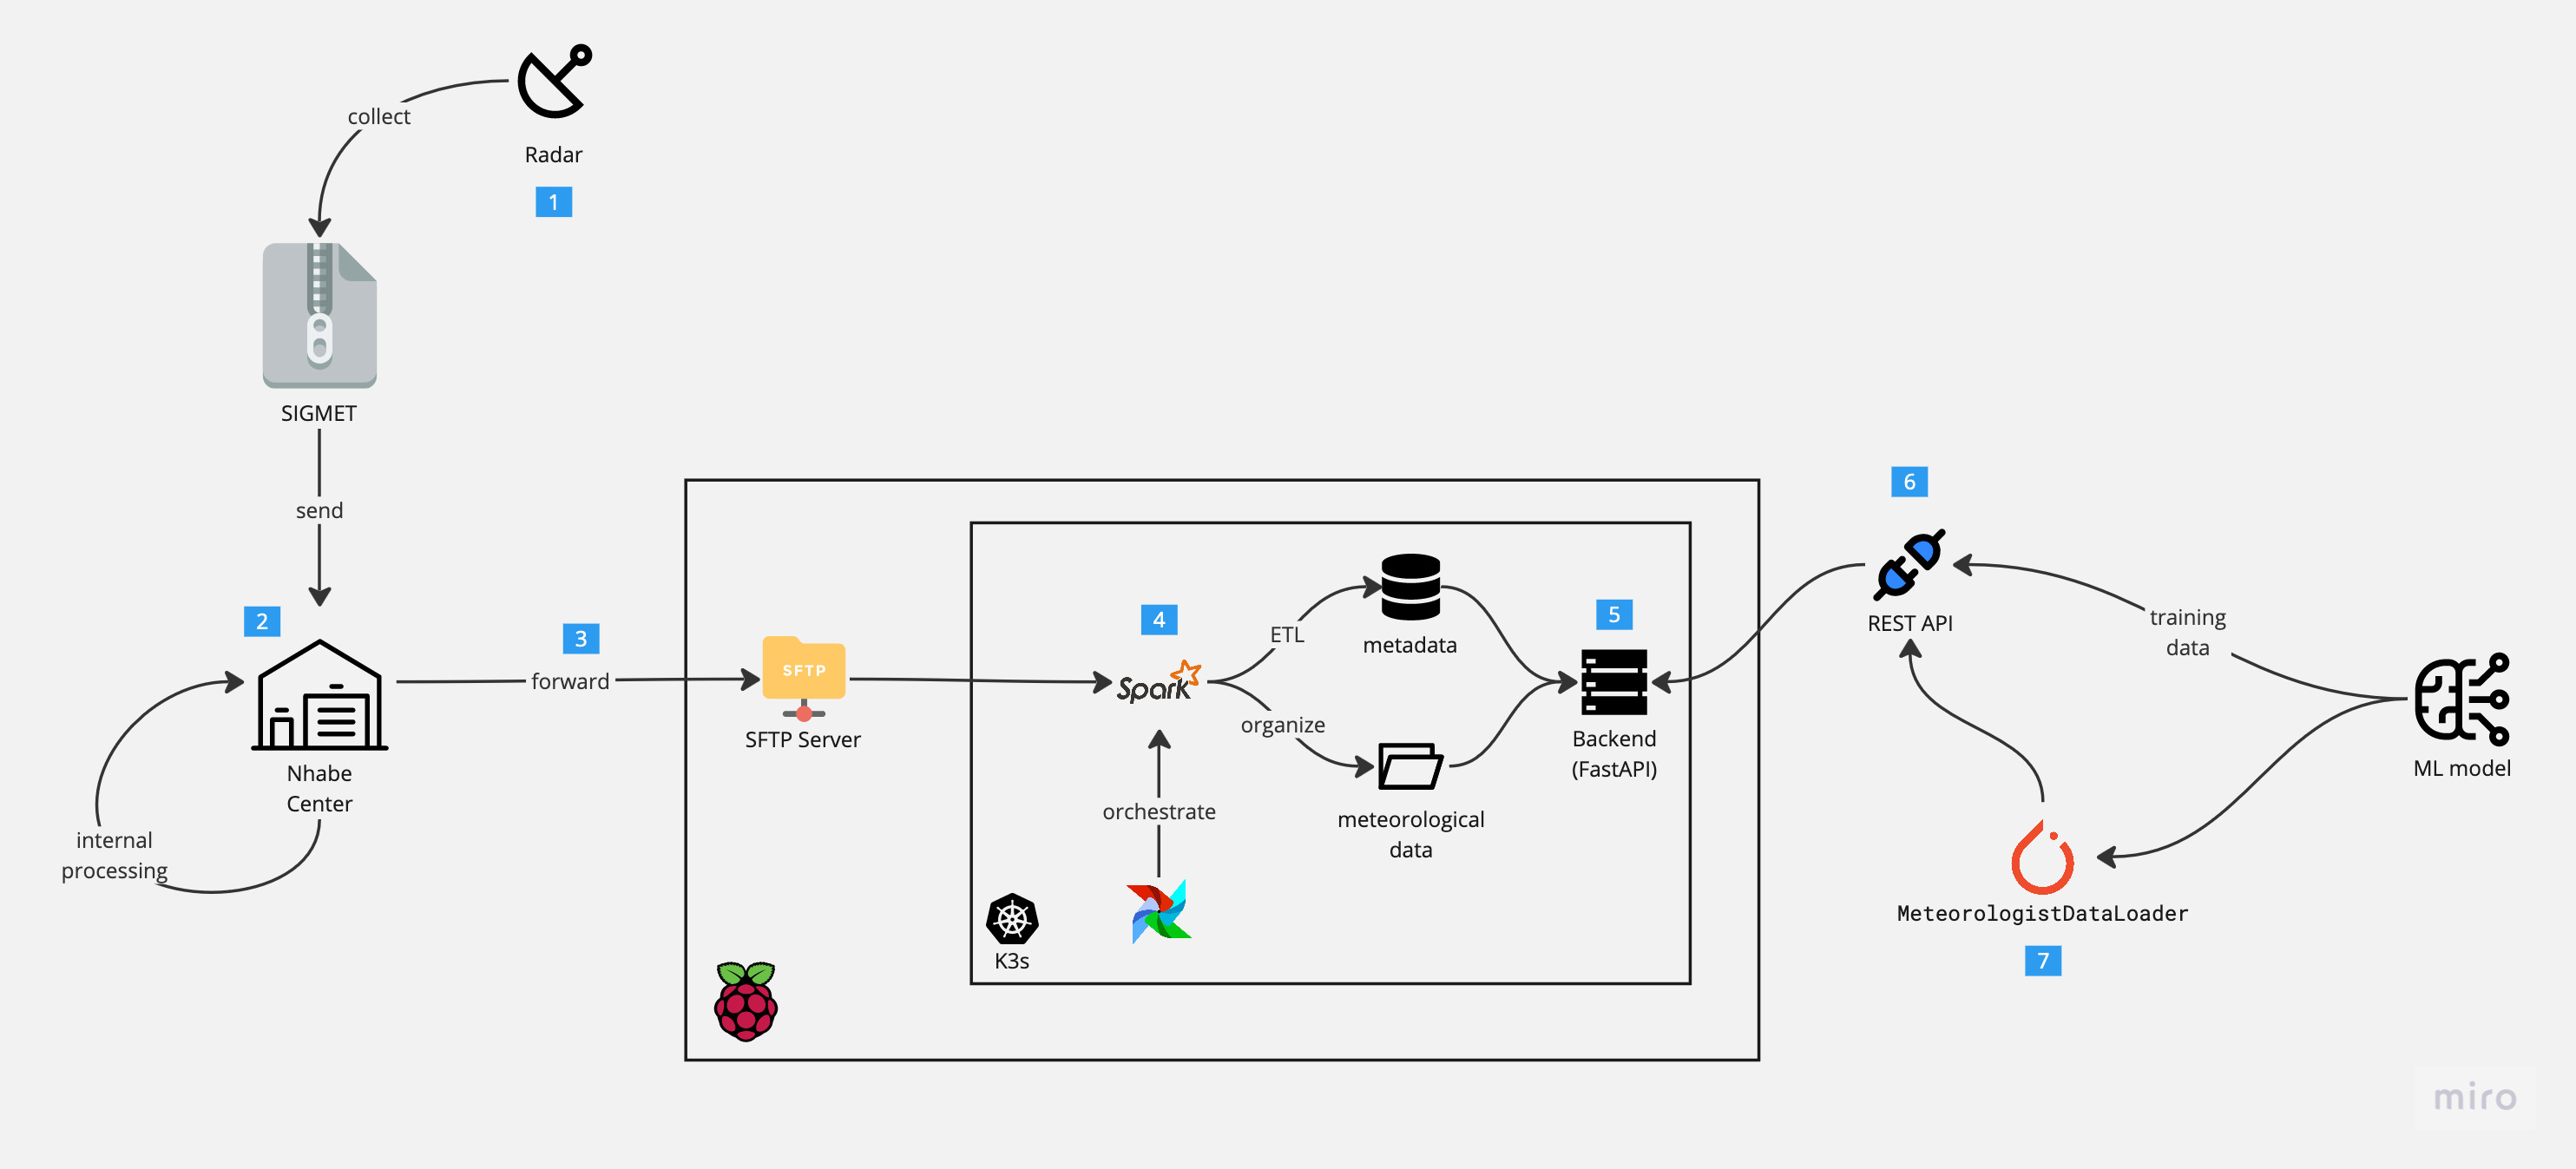
\includegraphics[width=\linewidth]{Images/4.1-architecture.jpg}
    \vspace{1em}
    \caption{System Design - Proposed}
    \label{fig:sow}
\end{figure}
\vspace{0.5cm}
Based on the requirements set by stakeholders and after studying the existing system, the team proposes the design and implementation of a system titled "Integrated Database for Short-Term Prediction in Hydrometeorology." Figure \ref{fig: sow} illustrates the team's design template.
\newpage
\section{Current System}
The design comprises seven main sections. Among them, the part of the system currently operational at the Nha Be observation station is depicted in the first two steps:

Firstly, in step 1, during each specific cycle, a geostationary satellite collects meteorological data. Some received indices include:
\begin{enumerate}
    \item Doppler Spectrum Width
    \item Mean Doppler Velocity
    \item Reflectivity
\end{enumerate}

All this information is transmitted to the Nha Be observation station in the SIGMET format \ref{sigmet}. Subsequently, in step 2, the meteorological staff at the Nha Be station records and processes the transmitted data according to their operational requirements.
